\section{Theorie}
\label{sec:Theorie}

Als geometrische Optik (auch Strahlenoptik) wird der Teilbereich der Optik bezeichet, in welchem angenommen wird, dass Licht sich strahlenförmig und geradlinig ausbreitet.
Dies ist eine Nährung der Wellenoptik und ist nur dann sinnvoll zu betrachten, wenn die betrachtete Strahlung eine kleine Wellenlänge und keine Welleneffekte aufzeigt.
Die hier hauptsächlich auftretenden Effekte sind die Reflexion und die Brechung.

In diesem Versuch wird nur die Brechung untersucht.
Im Brechungsgesetz nach Snellius
\begin{equation}
    n_1 \sin \alpha_1 = n_2 \sin \alpha_2
    \label{eq:brechungsgesetz}
\end{equation}
sind $n_1$ und $n_2$ die Brechungsindizes des beiden betrachteten Materialien.
Hierrüber wird beschrieben wie Licht sich an einer Grenzfläche von zwei verschiedenen Medien verhält.
Dabei sind $\alpha_1$ und $\alpha_2$ die Winkel der Lichtstrahlen zum Lot auf die Fläche.

Hierfür wird untersucht inwiefern Linsen den Strahlengang von sichtbarem Licht beinflussen.
Linsen sind lichtdurchlässige Objekte, die meistens eine rotationssymmetrische gekrümmte Oberfläche und einen höheren Brechungsindex als Luft haben.

\begin{figure}
    \centering
    \begin{subfigure}{0.4\textwidth}
        \centering
        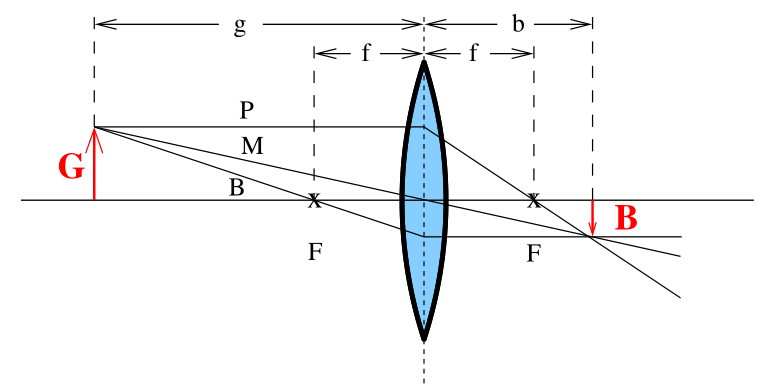
\includegraphics[width=\textwidth]{images/skizze_linse_1.png}
        \caption{Sammellinse}
        \label{fig:skizze_linse_1}
    \end{subfigure}    
    \begin{subfigure}{0.4\textwidth}
        \centering
        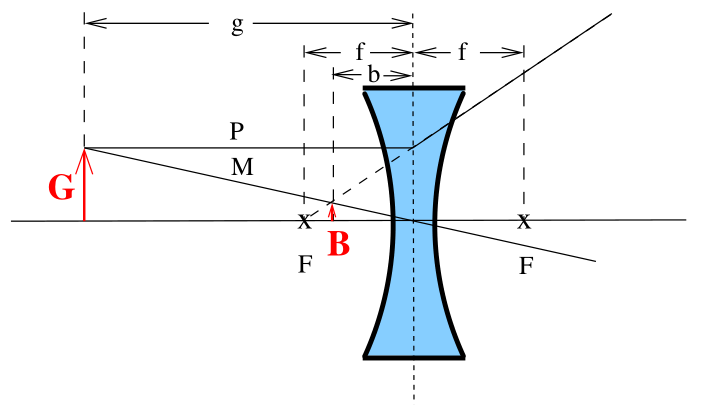
\includegraphics[width=\textwidth]{images/skizze_linse_2.png}
        \caption{Zerstreuungslinse}
        \label{fig:skizze_linse_2}
    \end{subfigure}    
    \caption{Skizze der beiden Hauptarten von Linsen mit bezeichnungen aller nötigen Abstände. \cite{V408}}
    \label{fig:linsenarten}
\end{figure}

Grunsätzlich wird zwischen zwei Linsenarten unterschieden. (siehe \autoref{fig:linsenarten})
Sammellinsen bündeln alle von einem Punkt ausgehenden Lichtstrahlen in einem Punkt auf der anderen Seite der Linse.
Somit wird ein (reelles) Bild erzeugt, das auf einem Schirm sichtbar gemacht werden kann.

Als Brennpunkt oder auch Fokus $F$ wird der Punkt bezeichnet in dem sich alle parallel auf die Linse eintreffenden Strahlen bündeln.

Zerstreuungslinsen hingegen brechen die Lichtstrahlen so, dass diese sich hinter der Linse noch weiter voneinander entfernen.
Bei Zerstreuungslinsen liegt der Brennpunkt vor der Linse, da alle parallel eintreffenden Strahlen so gebrochen werden, als wäre der Fokus ihr Ursprung.
Somit wäre auch der Bildpunkt vor der Linse und es wird von einem virtuellen Bild gesprochen. (vgl. \autoref{fig:skizze_linse_2})

Eigentlich wird der Lichtstrahl bei einer Linse an zwei gekrümmten Grenzflächen gebrochen. 
Um diese komplexe Brechung einfacher beschreiben zu können werden zwei Hauptebenen eingezeichnet, die das Brechungsverhalten charakterisieren. 
Zwischen den Hauptflächen wird angenommen dass der Lichtstrahl parallel zur optischen Achse verläuft. (vgl. \autoref{fig:skizze_linse_3})
Ist die betrachtete Linse dünn genug, so werden die zwei Hauptebenen zu einer Hauptebene. (vgl. \autoref{fig:linsenarten})

\begin{figure}
    \centering
    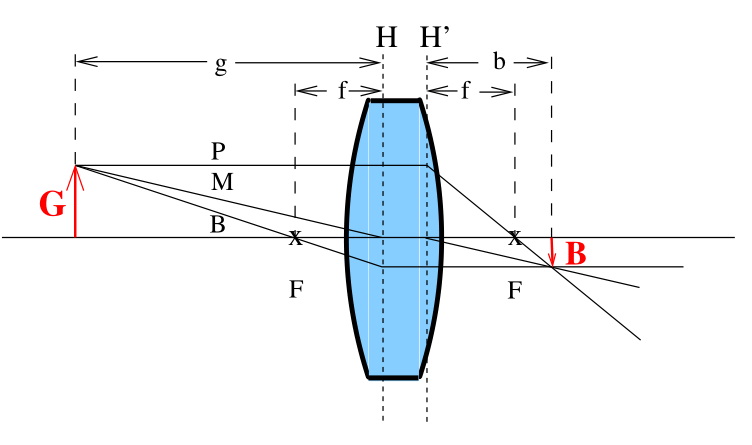
\includegraphics[width=0.4\textwidth]{images/skizze_linse_3.png}
    \caption{Skizze einer dickeren Sammellinse, welche zwei Hauptebenen benötigt.\cite{V408}}
    \label{fig:skizze_linse_3}
\end{figure}

Die Brennweite $f$ ist der Abstand von einer Hauptebene zum entsprechenden Brennpunkt. 
Sie ist eine Konstante, die die Brechung einer Linse charakterisiert.

Der Abstand von der Hauptebene zum Bild ist die sogenannte Bildweite $b$.
Und der Abstand von der anderen Hauptebene zum Abgebildeten Objekt ist die Gegenstandsweite $g$.

Um zeichnerisch das Bild zu konstruieren werden drei Strahlen eingezeichnet: Der Parallelstrahl P, der Mittelpunktstrahl M und der Brennpunktstrahl B. 
Mithilfe dieser Strahlen und den Strahlensätzen lässt sich der Zusammenhang
\begin{equation}
    V \coloneqq \frac{B}{G} = \frac{b}{g}
    \label{eq:abbildungsgesetz}
\end{equation}
aufstellen, welcher den Abbildungsmaßstab $V$ definiert und Abbildungsgesetz genannt wird.
Hierraus folgt das sogenannte Linsengesetz
\begin{equation}
    \frac{1}{f} = \frac{1}{b} + \frac{1}{g} \, .
    \label{eq:linsengesetz}
\end{equation}

Das Vereinfachen der Brechung von Linsen auf zwei Hauptebenen gilt nur bei Strahlen die nahe der optischen Achse verlaufen.
Durch achsenferne Strahlen kommen Abbildungsfehler zustande und das Bild wird unscharf, weil diese Strahlen einen nähreren Brennpunkt aufweisen, als achsennahe Strahlen.
Dieser Effekt wird auch sphärische Abberation genannt und kann unter Verwendung einer Blende korrigiert werden, da so achsenferne Strahlen nicht die Linse erreichen.

Eine weitere Quelle von Abbildungsfehlern ist die Dispersion.
Der Brechungsindex ist abhängig von der Wellenlänge des Lichts.
Blaues Licht (kurze Wellenlänge) wird mehr gebrochen als rotes Licht (lange Wellenlänge).
Dadurch entsteht des Effekt der chromatischen Abberation und der Brennpunkt von blauem Licht liegt näher an der Linse als der Brennpunkt von rotem Licht.

Betrachtet man ein System aus mehreren Linsen können die Brechkräfte $D=1/f$ der einzelnen Linsen einfach aufsummiert werden.
